%% V1.0
%% by Gabriel Garcia, gabrcg@gmail.com
%% This is a template for Udacity projects using IEEEtran.cls

%% Be Udacious!

\documentclass[10pt,journal,compsoc]{IEEEtran}

\usepackage[pdftex]{graphicx}    
\usepackage{cite}
\hyphenation{op-tical net-works semi-conduc-tor}


\begin{document}

\title{Slam In Robotics}

\author{Mahmoud Selim}

\markboth{SLAM project, Robotic Nanodegree, Udacity, RTAB-Mapping, Robotics}%
{}
\IEEEtitleabstractindextext{%

\begin{abstract}
In Robotics, localization and mapping are the key skills that enable robots to interact with their environment, by being able
to locate itself relative to the map of previously visited locations. Mapping a location (e.g. an apartment room or an outdoor area) from
sensor data while locating oneself in that consistently updating environment is referred to as Simultaneous Localization And Mapping
(SLAM). In this project the SLAM implementation of Real-Time Appearance Based Mapping (RTABMap) is done through the
rtabmap_ros package and implemented on a teleoperated robot to map 2 simulated worlds made in Gazebo. Both worlds were
successfully mapped, which allows for a first look at some considerations to be made when attempting to map an environment using
robots.
\end{abstract}

% Note that keywords are not normally used for peerreview papers.
\begin{IEEEkeywords}
Robot, IEEEtran, Udacity, deep learning.
\end{IEEEkeywords}}


\maketitle
\IEEEdisplaynontitleabstractindextext
\IEEEpeerreviewmaketitle
\section{Introduction}
\label{sec:introduction}

\IEEEPARstart{T}{he} goal of this project is to perform simultaneos localization and mapping for two environments using the RTABMap algorithm implemented on. SLAM in
robotics enables a robot to map an environment and also to keep track of the position relative to the environment it
is in.
More often than not, the architect blueprint of a building
is inaccurate, and even in the event that it was perfectly
accurate, the addition of furniture would alter the ”map” of
the building by the robot, since if it were to perform a task
within that environment, it would need to know about the
position of this furniture.
This problem is interesting because it implies that every building needs to be mapped if a robot is going to do anything
autonomously within these buildings. This statement can be pushed further to
encompass any kind of environments. However in the ideal situation, the 
robot will adapt it's map when slight changes occurs within it.
Therefore, if one can make a robot able to navigate and
sense it's surroundings, then these environments should be mapped.

Potential applications can go from mapping an office
layout for automated cleaning, mapping a suburb for civil
engineers to design upgrades to a city, to mapping a region
of the moon for installing a base on the moon. The importance of mapping is similar to how important it is for humans
to remember places they’ve been to. Thus, it is a crucial part for any mobile robot to not only be able to map its environment, but also to adjust these maps when changes occurs to them.



\section{BACKGROUND}
\subsection{Mapping in Robotics}
Mapping in Robotics is used to enable the robot to model the environment it is in. Locating the robot with respect
to its environment requires a map of the environment, and
mapping requires the robot’s pose, which is obtained during
the localization. This is a typical scenario for the ”chicken and the egg”
problem, where location requires a map of the environment to be referenced to
and mapping requires the location of the robot.
\subsection{SLAM}
Simultaneous Localization and Mapping (SLAM) solves this
problem by simultaneously and iteratively computing the
map (m) and robot’s pose (x_t) from sensory and odometric measurements (z_t), control actions (u_t), and correspondences (c_t) between features within the map. There are two
different variants of SLAM:
\begin{itemize}
\item Online SLAM: it solves the SLAM problem by only
looking at the current pose and local correspondences to estimate the robot’s pose and update the
map: P(x_t, m, c_t|u_{1:t}, z_{1:t}).
\item Full SLAM: Unlike the Online SLAM, Full SLAM,
also referred to Offline SLAM, takes into account all
poses and map correspondences to estimate the pose
and update the map: P(x_{1:t}, m, c_{1:t}|u_{1:t}, z_{1:t}).
\end {itemize}
There exist different implementations of the SLAM algorithm, examples for these might be FastSLAM, Grid-Based
SLAM, and Graph SLAM.

\paragraph FastSLAM estimates the pose of the robot using particles, like the Monte Carlo Localization algorithm and builds
the map using an EKF to solve the independent features
of the map as local Gaussians. The main disadvantage of
this approach is that it always need to assume that there
are known landmarks within the map, and therefore it is
impossible to model an arbitrary environment.
\paragraph Grid-Based SLAM is a variant of FastSLAM which
updates the map using grids, like the Occupancy Grid Mapping algorithm, in order to fix the previously mentioned
issues with the FastSLAM algorithm. Grid-Based SLAM,
like FastSLAM uses a particle filter to estimates the pose
\paragraph GraphSLAM on the other hand aims create a graph of
robot poses and map features and attempts to minimize the
over error between all motion and measurement constraints.

\subsection{RTABMap}
\subsubsection{General Description}
Real-Time Appearance Based Mapping (RTABMap) or Appearance Based SLAM implements GraphSLAM by collecting data from visual sensors to locate the robot and map the
environment. SLAM with RTABMap can be separated into
two parts: the front-end, which uses sensory and odometric data to create a graph with loop closure constraints; the
second part, the back-end, handles the graph optimization
and the 2D/3D mapping.

\begin{figure}[thpb]
      \centering
      \includegraphics[width=\linewidth]{graph_slam5}
      \caption{Graph SLAM Nodes.}
      \label{fig: Graph SLAM}
\end{figure}


\subsubsection{Loop closure and bag-of-words}
RTABMap uses loop closure to determine whether a robot
has seen a location before. RTABMap uses Speeded Up
Robust Features (SURF) to extract features and describe
them with a unique representations then it clusters similar
or synonym features together and name them to create
vocabulary. One of the feature description is then mapped
to one the vocabulary, it is called quantization. Features are
now linked to a word and can be referred to as a visual
word. When all features in an image are quantized, the
image is now a bag-of-words. To compare an image with
previously seen images, a matching score is given to all
images containing the same words using a bayesian filter,
and similar images can be found, this is called an inverted
index. Finally if the current image contains similar words to
that of a previously seen image (bag-of-words) it will have
a higher score, and if the score reaches a threshold H, a loop
closure is detected
\begin{figure}[thpb]
      \centering
      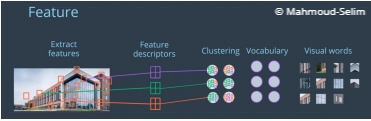
\includegraphics[width=\linewidth]{bag_of_words}
      \caption{ Features are extracted and a bag-of-words is created from an image}
      \label{fig:bow}
\end{figure}

\subsubsection{Memory management}
RTABMap uses a memory management technique to limit
the number of locations considered as candidates during
loop-closure detection, which allows it to be done in RealTime. The technique can be summarized as follows: it
keeps the most frequently observed locations in the robot’s
working memory (WM) and transfers other images to the
long term memory (LTM). When an image is first acquired
a new node is created in the short term memory (STM),
features are then extracted and a it is then compared to the
vocabulary to find all of the words in the image, creating
a bag-of-word for this node. Nodes are assigned a weight
in the STM based on how long the robot spent in the location, the longer, the higher the weight. STM has a fixed
size S, when the STM reaches S nodes the oldest node is
transferred to the WM to be considered for loop closure
detection. WM size depends on a fixed time T, and when
the time required to process new data reaches T, then some
nodes are transferred to the LTM. Finally if a loop closure is
detected, neighbour nodes in the LTM are transferred to the
WM.
\begin{figure}[thpb]
      \centering
      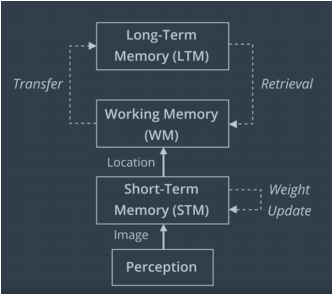
\includegraphics[width=\linewidth]{memory_management}
      \caption{ RTAB-MAP Memory Management}
      \label{fig:rtab_mem_mgmt}
\end{figure}


\section{SCENE AND MODEL CONFIGURATION}
\subsubsection{Robot Configuration}
RTABMap uses a memory management technique to limit
the number of locations considered as candidates during
loop-closure detection, which allows it to be done in RealTime. The technique can be summarized as follows: it
keeps the most frequently observed locations in the robot’s
working memory (WM) and transfers other images to the
long term memory (LTM). When an image is first acquired
a new node is created in the short term memory (STM),
features are then extracted and a it is then compared to the
vocabulary to find all of the words in the image, creating
a bag-of-word for this node. Nodes are assigned a weight
in the STM based on how long the robot spent in the location, the longer, the higher the weight. STM has a fixed
size S, when the STM reaches S nodes the oldest node is
transferred to the WM to be considered for loop closure
detection. WM size depends on a fixed time T, and when
the time required to process new data reaches T, then some
nodes are transferred to the LTM. Finally if a loop closure is
detected, neighbour nodes in the LTM are transferred to the
WM.
\begin{figure}[thpb]
      \centering
      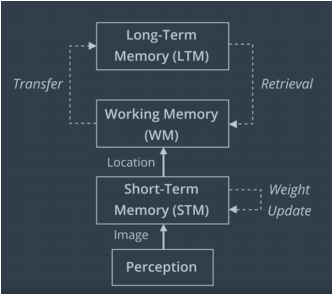
\includegraphics[width=\linewidth]{memory_management}
      \caption{ RTAB-MAP Memory Management}
      \label{fig:rtab_mem_mgmt}
\end{figure}



\subsubsection{}
Subsubsection text here.


\begin{table}[h]
\caption{Table}
\label{table_example}
\begin{center}
\begin{tabular}{|c||c|}
\hline
One & Two\\
\hline
Three & Four\\
\hline
\end{tabular}
\end{center}
\end{table}



   

\section{Background / Formulation}
At this stage, you should begin diving into the technical details of your approach by explaining to the reader how parameters were defined, what type of network was chosen, and the reasons these items were performed. This should be factual and authoritative, meaning you should not use language such as “I think this will work” or “Maybe a network with this architecture is better..”. Instead, focus on items similar to, ”A 3-layer network architecture was chosen with X, Y, and Z parameters” 
Explain why you chose the network you did for the supplied data set and then why you chose the network used for your robotic inference project. \cite{lamport1994latex}

%example for Bullet point list

\begin{itemize}
\item example
\end {itemize}



%example for numbered list
\begin{enumerate}
\item example

\end{enumerate}

\section{Data Acquisition}
This section should discuss the data set. Items to include are the number of images, size of the images, the types of images (RGB, Grayscale, etc.), how these images were collected (including the method). Providing this information is critical if anyone would like to replicate your results. After all, the intent of reports such as these are to convey information and build upon ideas so you want to ensure others can validate your process.
Justifying why you gathered data in this way is a helpful point, but sometimes this may be omitted here if the problem has been stated clearly in the introduction.
It is a great idea here to have at least one or two images showing what your data looks like for the reader to visualize.

\section{Results}
This is typically the hardest part of the report for many. You want to convey your results in an unbiased fashion. If you results are good, you can objectively note this. Similarly, you may do this if they are bad as well. You do not want to justify your results here with discussion; this is a topic for the next session. 
Present the results of your robotics project model and the model you used for the supplied data with the appropriate accuracy and inference time
For demonstrating your results, it is incredibly useful to have some charts, tables, and/or graphs for the reader to review. This makes ingesting the information quicker and easier.

\section{Discussion}
This is the only section of the report where you may include your opinion. However, make sure your opinion is based on facts. If your results are poor, make mention of what may be the underlying issues. If the results are good, why do you think this is the case? Again, avoid writing in the first person (i.e. Do not use words like “I” or “me”). If you really find yourself struggling to avoid the word “I” or “me”; sometimes, this can be avoid with the use of the word “one”. As an example: instead of : “I think the accuracy on my dataset is low because the images are too small to show the necessary detail” try: “one may believe the accuracy on the dataset is low because the images are too small to show the necessary detail”. They say the same thing, but the second avoids the first person. 
Reflect on which is more important, inference time or accuracy, in regards to your robotic inference project.

\section{Conclusion / Future work}
This section is intended to summarize your report. Your summary should include a recap of the results, did this project achieve what you attempted, and is this a commercially viable product? 
For Future work,address areas of work that you may not have addressed in your report as possible next steps. For future work, this could be due to time constraints, lack of currently developed methods / technology, and areas of application outside of your current implementation. Again, avoid the use of the first-person.

\bibliography{bib}
\bibliographystyle{ieeetr}

\end{document}